


\label{experiment-perl.tex}

\section{
Experiment Management System}






      {\bf $\bullet$} Introduction (page \pageref{experiment-perl.texntoc1}) 

      {\bf $\bullet$} Requirements (page \pageref{experiment-perl.texntoc2}) 

      {\bf $\bullet$} Quick Start (page \pageref{experiment-perl.texntoc3}) 

      {\bf $\bullet$} More Examples (page \pageref{experiment-perl.texntoc4}) 

      {\bf $\bullet$} Phrase Model (page \pageref{experiment-perl.texntoc5}) 

      {\bf $\bullet$} Factored Phrase Model (page \pageref{experiment-perl.texntoc6}) 

      {\bf $\bullet$} Hierarchical model (page \pageref{experiment-perl.texntoc7}) 

      {\bf $\bullet$} Target syntax model (page \pageref{experiment-perl.texntoc8}) 

      {\bf $\bullet$} Try a Few More Things (page \pageref{experiment-perl.texntoc9}) 

      {\bf $\bullet$} Stemmed Word Alignment (page \pageref{experiment-perl.texntoc10}) 

      {\bf $\bullet$} Using Multi-Threaded GIZA++ (page \pageref{experiment-perl.texntoc11}) 

      {\bf $\bullet$} Using Berkeley Aligner (page \pageref{experiment-perl.texntoc12}) 

      {\bf $\bullet$} IRST Language Model (page \pageref{experiment-perl.texntoc13}) 

      {\bf $\bullet$} Randomized Language Model (page \pageref{experiment-perl.texntoc14}) 

      {\bf $\bullet$} Compound Splitting (page \pageref{experiment-perl.texntoc15}) 

      {\bf $\bullet$} A Short Manual (page \pageref{experiment-perl.texntoc16}) 

      {\bf $\bullet$} Experiment.Meta (page \pageref{experiment-perl.texntoc17}) 

      {\bf $\bullet$} Multiple Corpora, One Translation Model (page \pageref{experiment-perl.texntoc18}) 

      {\bf $\bullet$} Defining Settings (page \pageref{experiment-perl.texntoc19}) 

      {\bf $\bullet$} Working with Experiment.Perl (page \pageref{experiment-perl.texntoc20}) 

      {\bf $\bullet$} Continuing Crashed Experiments (page \pageref{experiment-perl.texntoc21}) 

      {\bf $\bullet$} Running on a Cluster (page \pageref{experiment-perl.texntoc22}) 

      {\bf $\bullet$} Running on a Multicore Machine (page \pageref{experiment-perl.texntoc23}) 

      {\bf $\bullet$} Web Interface (page \pageref{experiment-perl.texntoc24}) 

      {\bf $\bullet$} Analysis (page \pageref{experiment-perl.texntoc25})






\subsection{
\label{experiment-perl.texntoc1}Introduction}


The Experiment Management System (EMS), or Experiment.perl, for lack of a better name, makes it much easier to perform experiments with Moses.



There are many steps in running an experiment: the preparation of training data, building language and translation models, tuning, testing, scoring and analysis of the results. For most of these steps, a different tool needs to be invoked, so this easily becomes very messy.



Here a typical example:









\begin{center}
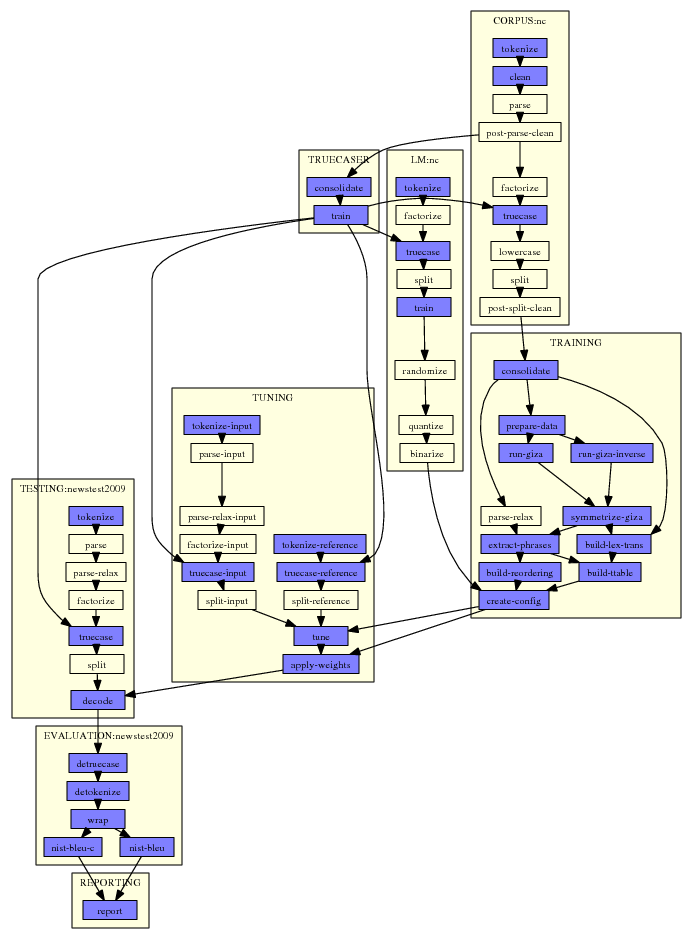
\includegraphics[scale=0.5]{images/ems-agenda.png}
\end{center}




This graph was automatically generated by Experiment.perl. All that needed to be done was to specify one single configuration file that points to data files and settings for the experiment.



In the graph, each step is a small box. For each step, Experiment.perl builds a script file that gets either submitted to the cluster or run on the same machine. Note that some steps are quite involved, for instance tuning: On a cluster, the tuning script runs on the head node a submits jobs to the queue itself.



Experiment.perl makes it easy to run multiple experimental runs with different settings or data resources. It automatically detects which steps do not have to be executed again but instead which results from an earlier run can be re-used.



Experiment.perl also offers a web interface to the experimental runs for easy access and comparison of experimental results.









\begin{center}
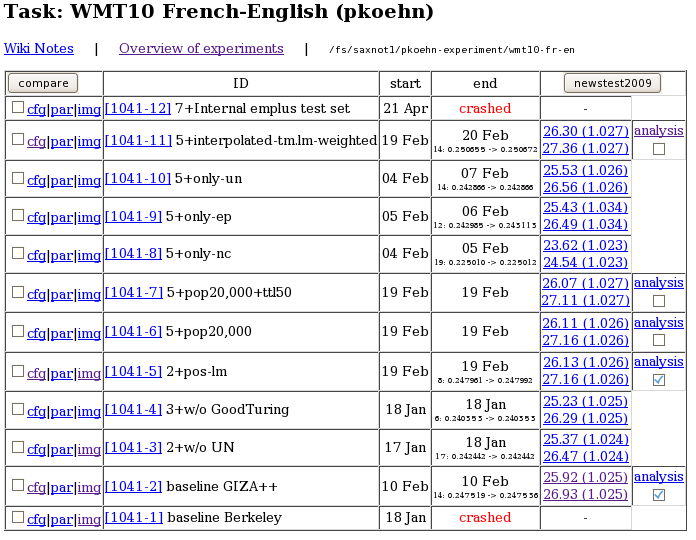
\includegraphics[scale=0.5]{images/ems-web.png}
\end{center}




The web interface also offers some basic analysis of results, such as comparing the n-gram matches between two different experimental runs:









\begin{center}
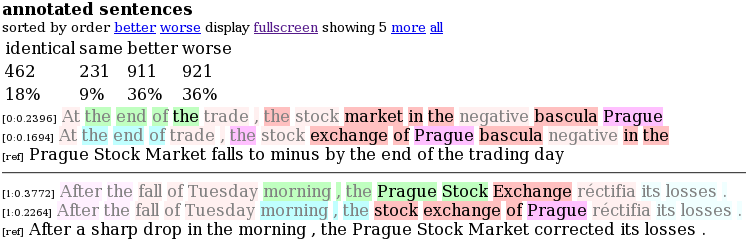
\includegraphics[scale=0.5]{images/ems-analysis.png}
\end{center}




\subsection{
\label{experiment-perl.texntoc2}Requirements}


In order to run properly, EMS will require:

\begin{itemize}
\item A version of Moses along with SRILM

\item The GraphViz toolkit\footnote{\sf http://www.graphviz.org/}.

\item The ImageMagick toolkit\footnote{\sf http://www.imagemagick.org/script/index.php}.

\item The GhostView tool\footnote{\sf http://www.gnu.org/software/gv/}.

\end{itemize}

\subsection{
\label{experiment-perl.texntoc3}Quick Start}


Experiment.perl is extremely simple to use:

\begin{itemize}
\item Find {\tt experiment.perl} in {\tt scripts/ems}

\item Get a sample configuration file from someplace (for instance {\tt scripts/ems/example/config.toy}).

\item Set up a working directory for your experiments for this task ({\tt mkdir} does it).

\item Edit the following path settings in {\tt config.toy}
\begin{itemize}
\item {\tt working-dir}

\item {\tt data-dir}

\item {\tt moses-script-dir}

\item {\tt moses-src-dir}

\item {\tt srilm-dir}

\item {\tt decoder}

\end{itemize}

\item Run {\tt experiment.perl -config config.toy} from your experiment working directory.

\item Marvel at the graphical plan of action.

\item Run {\tt experiment.perl -config config.toy -exec}.

\item Check the results of your experiment (in {\tt evaluation/report.1})

\end{itemize}

Let us take a closer look at what just happened.



The configuration file {\tt config.toy} consists of several sections. For instance there is a section for each language model corpus to be used. In our toy example, this section contains the following:






\begin{SaveVerbatim}{myverb}
 [LM:toy]

 ### raw corpus (untokenized)
 #
 raw-corpus = $toy-data/nc-5k.$output-extension
\end{SaveVerbatim}
\colorbox{gray}{%
\BUseVerbatim{myverb}
}

The setting {\tt raw-corpus} species the location of the corpus. The definition uses the variables {\tt \$toy-data} and {\tt \$output-extension}, which are also settings defined elsewhere in the configuration file. These variables are resolved, leading to the file path {\tt ems/examples/data/nc-5k.en} in your Moses scripts directory.



The authoritative definition of the steps and their interaction is in the file {\tt experiment.meta} (in the same directory as experiment.perl: {\tt scripts/ems}). 



The logic of {\tt experiment.meta} is that it wants to create a report at the end. To generate the report it needs to evaluation scores, to get these it needs decoding output, to get these it needs to run the decoder, to be able to run the decoder it needs a trained model, to train a model it needs data. This process of defining the agenda of steps to be executed is very similar to the Make utility in Unix.



We can find the following step definitions for the language model module in {\tt experiment.meta}:






\begin{SaveVerbatim}{myverb}
 get-corpus
        in: get-corpus-script
        out: raw-corpus
        default-name: lm/txt
        template: IN > OUT
 tokenize
        in: raw-corpus
        out: tokenized-corpus
        default-name: lm/tok
        pass-unless: output-tokenizer
        template: $output-tokenizer < IN > OUT
        parallelizable: yes
\end{SaveVerbatim}
\colorbox{gray}{%
\BUseVerbatim{myverb}
}

The tokenization step {\tt tokenize} requires {\tt raw-corpus} as input. In our case, we specified the setting in the configuration file. We could have also specified an already tokenized corpus with {\tt tokenized-corpus}. This would allow us to skip the tokenization step. Or, to give another example, we could have not specified {\tt raw-corpus}, but rather specify a script that generates the corpus with the setting {\tt get-corpus-script}. This would have triggered the creation of the step {\tt get-corpus}.



The steps are linked with the definition of their input {\tt in} and output {\tt out}. Each step has also a default name for the output ({\tt efault-name}) and other settings.



The tokenization step has as default name {\tt lm/tok}. Let us look at the directory {\tt lm} to see which files it contains:






\begin{SaveVerbatim}{myverb}
 % ls -tr lm/*
 lm/toy.tok.1
 lm/toy.truecased.1
 lm/toy.lm.1
\end{SaveVerbatim}
\colorbox{gray}{%
\BUseVerbatim{myverb}
}

We find the output of the tokenization step in the file {\tt lm/toy.tok.1}. The {\tt toy} was added from the name definition of the language model (see {\tt [LM:toy]} in {\tt config.toy}). The {\tt 1} was added, because this is the first experimental run.



The directory {\tt steps} contains the script that executes each step, its STDERR and STDOUT output, and meta information. For instance:






\begin{SaveVerbatim}{myverb}
 % ls steps/1/LM_toy_tokenize.1* | cat
 steps/1/LM_toy_tokenize.1
 steps/1/LM_toy_tokenize.1.DONE
 steps/1/LM_toy_tokenize.1.INFO
 steps/1/LM_toy_tokenize.1.STDERR
 steps/1/LM_toy_tokenize.1.STDERR.digest
 steps/1/LM_toy_tokenize.1.STDOUT
\end{SaveVerbatim}
\colorbox{gray}{%
\BUseVerbatim{myverb}
}

The file {\tt steps/2/LM\_toy\_tokenize.2} is the script that is run to execute the step. The file with the extension {\tt DONE} is created when the step is finished - this communicates to the scheduler that subsequent steps can be executed. The file with the extension {\tt INFO} contains meta information - essential the settings and dependencies of the step. This file is checked to detect if a step can be re-used in new experimental runs.



In case that the step crashed, we expect some indication of a fault in {\tt STDERR} (for instance the words {\tt core dumped} or {\tt killed}). This file is checked to see if the step was executed successfully, so subsequent steps can be scheduled or the step can be re-used in new experiments. Since the {\tt STDERR} file may be very large (some steps create Megabytes of such output), a digested version is created in {\tt STDERR.digest}. If the step was successful, it is empty. Otherwise it contains the error pattern that triggered the failure detection.



Let us now take a closer look at re-use. If we run the experiment again but change some of the settings, say, the order of the language model, then there is no need to re-run the tokenization. 



Here is the definition of the language model training step in {\tt experiment.meta}:






\begin{SaveVerbatim}{myverb}
 train
        in: split-corpus
        out: lm
        default-name: lm/lm
        ignore-if: rlm-training
        rerun-on-change: lm-training order settings
        template: $lm-training -order $order $settings -text IN -lm OUT
        error: cannot execute binary file
\end{SaveVerbatim}
\colorbox{gray}{%
\BUseVerbatim{myverb}
}

The mention of {\tt order} in the list behind {\tt rerun-on-change} informs experiment.perl that this step does need to be re-run, of the order of the language model changes. Since none of the settings in the chain of steps leading up to the training have been changed, the can be re-used.



Try changing the language model order ({\tt order = 5} in {\tt config.toy}), run experiment.perl again ({\tt experiment.perl -config config.toy}) in the working directory, and you will see the new language model in the directory {\tt lm}:






\begin{SaveVerbatim}{myverb}
 % ls -tr lm/*
 lm/toy.tok.1
 lm/toy.truecased.1
 lm/toy.lm.1
 lm/toy.lm.2
\end{SaveVerbatim}
\colorbox{gray}{%
\BUseVerbatim{myverb}
}

\subsection{
\label{experiment-perl.texntoc4}More Examples}


The {\tt example} directory contains some additional examples. 



These require the training and tuning data released for the Shared Translation Task for WMT 2010.
Create a working directory, and change into it. Then execute the following steps:






\begin{SaveVerbatim}{myverb}
 mkdir data
 cd data
 wget://www.statmt.org/wmt10/training-parallel.tgz
 tar xzf training-parallel.tgz
 wget://www.statmt.org/wmt10/dev.tgz
 tar xzf dev.tgz
 cd ..
\end{SaveVerbatim}
\colorbox{gray}{%
\BUseVerbatim{myverb}
}

The examples using these corpora are

\begin{itemize}
\item {\tt config.basic} - a basic phrase based model

\item {\tt config.factored} - a factored phrase based model

\item {\tt config.hierarchical} - a hierarchical phrase based model

\item {\tt config.syntax} - a target syntax model

\end{itemize}

In all these example configuration files, most corpora are commented out. This is done by adding the word {\tt IGNORE} at the end of a corpus definition (also for the language models). This allows you to run a basic experiment with just the News Commentary corpus which finished relatively quickly. 
Remove the {\tt IGNORE} to include more training data. You may run into memory and disk space problems when using some of the larger corpora (especially the news language model), depending on your computing infrastructure.



If you decide to use multiple corpora for the language model, you may also want to try out interpolating the individual language models (instead of using them as separate feature functions). For this, you need to comment out the {\tt IGNORE} next to the {\tt [INTERPOLATED-LM]} section.



You may also specify different language pairs by changing the {\tt input-extension}, {\tt output-extension}, and {\tt pair-extension} settings.



Finally, you can run all the experiments with the different given configuration files and the data variations in the same working directory. The experimental management system figures out automatically which processing steps do not need to repeated because they can be re-used from prior experimental runs.



\vspace{2mm}

{\bf 
\label{experiment-perl.texntoc5}Phrase Model}


Phrase models are, compared to the following examples, the simplest models to be trained with Moses and the fastest models to run. You may prefer these models over the more sophisticated models whose added complexity may not justify the small (if any) gains.



The example {\tt config.basic} is similar to the toy example, except for a larger training and test corpora. Also, the tuning stage is not skipped. Thus, even with most of the corpora commented out, the entire experimental run will likely take a day, with most time taken up by word alignment ({\tt TRAINING\_run-giza} and {\tt TRAINING\_run-giza-inverse}) and tuning ({\tt TUNING\_tune}).



\vspace{2mm}

{\bf 
\label{experiment-perl.texntoc6}Factored Phrase Model}


Factored models allow for additional annotation at the word level which may be exploited in various models. The example in {\tt config.factored} uses part-of-speech tags on the English target side. 



Annotation with part-of-speech tags is done with MXPOST, which needs to be installed first. Please read the installation instructions\footnote{\sf http://www.statmt.org/moses/?n=Moses.ExternalTools\#mxpost}. After this, you can run experiment.perl with the configuration file {\tt config.factored}.



If compare the factored example {\tt config.factored} with the phrase-based example {\tt config.basic} you will notice the definition of the factors used:






\begin{SaveVerbatim}{myverb}
 ### factored training: specify here which factors used
 # if none specified, single factor training is assumed
 # (one translation step, surface to surface)
 #
 input-factors = word
 output-factors = word pos
 alignment-factors = "word -> word"
 translation-factors = "word -> word+pos"
 reordering-factors = "word -> word"
 #generation-factors = 
 decoding-steps = "t0"
\end{SaveVerbatim}
\colorbox{gray}{%
\BUseVerbatim{myverb}
}

the factor definition:






\begin{SaveVerbatim}{myverb}
 #################################################################
 # FACTOR DEFINITION

 [INPUT-FACTOR]

 # also used for output factors
 temp-dir = $working-dir/training/factor

 [OUTPUT-FACTOR:pos]

 ### script that generates this factor
 #
 mxpost = /home/pkoehn/bin/mxpost
 factor-script = "$moses-script-dir/training/wrappers/make-factor-en-pos.mxpost.perl -mxpost $mxpost"
\end{SaveVerbatim}
\colorbox{gray}{%
\BUseVerbatim{myverb}
}

and the specification of a 7-gram language model over part of speech tags:






\begin{SaveVerbatim}{myverb}
 [LM:nc=pos]
 factors = "pos"
 order = 7
 settings = "-interpolate -unk"
 raw-corpus = $wmt10-data/training/news-commentary10.$pair-extension.$output-extension
\end{SaveVerbatim}
\colorbox{gray}{%
\BUseVerbatim{myverb}
}

This factored model using all the available corpora is identical to the Edinburgh submission to the WMT 2010 shared task for English-Spanish, Spanish-English, and English-German language pairs (the French language pairs also used the $\text{10}^\text{9}$ corpus, the Czech language pairs did not use the POS language model, and German-English used additional pre-processing steps).



\vspace{2mm}

{\bf 
\label{experiment-perl.texntoc7}Hierarchical model}


Hierarchical phrase models allow for rules with gaps. Since these are represented by non-terminals and such rules are best processed with a search algorithm that is similar to syntactic chart parsing, such models fall into the class of tree-based or grammar-based models. For more information, please check the <a class='createlinktext' rel='nofollow' 
    href='http://www.statmt.org/moses/?n=Moses.SyntaxTutoral?action=edit'>Syntax Tutorial</a><a rel='nofollow' 
    class='createlink' href='http://www.statmt.org/moses/?n=Moses.SyntaxTutoral?action=edit'>?</a>.



From the view of setting up hierarchical models with experiment.perl, very little has to be changed in comparison to the configuration file for phrase-based models:






\begin{SaveVerbatim}{myverb}
 % diff config.basic config.hierarchical 
 33c33
 < decoder = $moses-src-dir/moses-cmd/src/moses
 ---
 > decoder = $moses-src-dir/moses-chart-cmd/src/moses_chart
 36c36
 < ttable-binarizer = $moses-src-dir/misc/processPhraseTable
 ---
 > #ttable-binarizer = $moses-src-dir/misc/processPhraseTable
 39c39
 < #ttable-binarizer = "$moses-src-dir/CreateOnDisk/src/CreateOnDiskPt 1 1 5 100 2"
 ---
 > ttable-binarizer = "$moses-src-dir/CreateOnDisk/src/CreateOnDiskPt 1 1 5 100 2"
 280c280
 < lexicalized-reordering = msd-bidirectional-fe
 ---
 > #lexicalized-reordering = msd-bidirectional-fe
 284c284
 < #hierarchical-rule-set = true
 ---
 > hierarchical-rule-set = true
 413c413
 < decoder-settings = "-search-algorithm 1 -cube-pruning-pop-limit 5000 -s 5000"
 ---
 > #decoder-settings = ""
\end{SaveVerbatim}
\colorbox{gray}{%
\BUseVerbatim{myverb}
}

The changes are: a different decoder binary (by default compiled into {\tt moses-chart-cmd/src/moses\_chart}) and {\tt ttable-binarizer} are used. The decoder settings for phrasal cube pruning do not apply. 
Also, hierarchical models do not allow for lexicalized reordering (their rules fulfill the same purpose), and the setting for hierarchical rule sets has to be turned on. The use of hierarchical rules is indicated with the setting {\tt hierarchical-rule-set}.



\vspace{2mm}

{\bf 
\label{experiment-perl.texntoc8}Target syntax model}


Syntax models imply the use of linguistic annotation for the non-terminals of hierarchical models. This requires running a syntactic parser. 



In our example {\tt config.syntax}, syntax is used only on the English target side. The syntactic constituents are labeled with Collins parser, which needs to be installed first. Please read the installation instructions\footnote{\sf http://www.statmt.org/moses/?n=Moses.ExternalTools\#collins}.



Compared to the hierarchical model, very little has to be changed in the configuration file:






\begin{SaveVerbatim}{myverb}
 % diff config.hierarchical config.syntax
 46a47,49
 > # syntactic parsers
 > collins = /home/pkoehn/bin/COLLINS-PARSER
 > output-parser = "$moses-script-dir/training/wrappers/parse-en-collins.perl"
 > 
 241c244
 < #extract-settings = ""
 ---
 > extract-settings = "--MinHoleSource 1 --NonTermConsecSource"
\end{SaveVerbatim}
\colorbox{gray}{%
\BUseVerbatim{myverb}
}

The parser needs to be specified, and the extraction settings may be adjusted. And you are ready to go.



\subsection{
\label{experiment-perl.texntoc9}Try a Few More Things}


\vspace{2mm}

{\bf 
\label{experiment-perl.texntoc10}Stemmed Word Alignment}


The factored translation model training makes it very easy to set up word alignment not based on the surface form of words, but any other property of a word. One relatively popular method is to use stemmed words for word alignment.



There are two reasons for this: For one, for morphologically rich languages, stemming overcome data sparsity problems. Secondly, GIZA++ may have difficulties with very large vocabulary sizes, and stemming reduces the number of unique words.



To set up stemmed word alignment in experiment.perl, you need to define a stem as a factor:






\begin{SaveVerbatim}{myverb}
 [OUTPUT-FACTOR:stem4]
 factor-script = "$moses-script-dir/training/wrappers/make-factor-stem.perl 4"

 [INPUT-FACTOR:stem4]
 factor-script = "$moses-script-dir/training/wrappers/make-factor-stem.perl 4"
\end{SaveVerbatim}
\colorbox{gray}{%
\BUseVerbatim{myverb}
}

and indicate the use of this factor in the {\tt TRAINING} section:






\begin{SaveVerbatim}{myverb}
 input-factors = word stem4
 output-factors = word stem4
 alignment-factors = "stem4 -> stem4"
 translation-factors = "word -> word"
 reordering-factors = "word -> word"
 #generation-factors = 
 decoding-steps = "t0"
\end{SaveVerbatim}
\colorbox{gray}{%
\BUseVerbatim{myverb}
}

\vspace{2mm}

{\bf 
\label{experiment-perl.texntoc11}Using Multi-Threaded GIZA++}


GIZA++ is one of the slowest steps in the training pipeline. Qin Gao implemented a multi-threaded version of GIZA++, called MGIZA, which speeds up word alignment on multi-core machines.



To use MGIZA, you will first need to install\footnote{\sf http://www.statmt.org/moses/?n=Moses.ExternalTools\#mgiza} it.



To use it, you simply need to add some training options in the section {\tt TRAINING}:






\begin{SaveVerbatim}{myverb}
 ### general options
 #
 training-options = "-mgiza -mgiza-cpus 8"
\end{SaveVerbatim}
\colorbox{gray}{%
\BUseVerbatim{myverb}
}

\vspace{2mm}

{\bf 
\label{experiment-perl.texntoc12}Using Berkeley Aligner}


The Berkeley aligner is a alternative to GIZA++ for word alignment. You may (or may not) get better results using this tool.



To use the Berkeley aligner, you will first need to install\footnote{\sf http://www.statmt.org/moses/?n=Moses.ExternalTools\#berkeley} it.



The example configuration file already has a section for the parameters for the tool. You need to un-comment them and adjust {\tt berkeley-jar} to your installation. You should comment out {\tt alignment-symmetrization-method}, since this is a GIZA++ setting.






\begin{SaveVerbatim}{myverb}
 ### symmetrization method to obtain word alignments from giza output
 # (commonly used: grow-diag-final-and)
 #
 #alignment-symmetrization-method = grow-diag-final-and

 ### use of berkeley aligner for word alignment
 #
 use-berkeley = true
 alignment-symmetrization-method = berkeley
 berkeley-train = $moses-script-dir/ems/support/berkeley-train.sh
 berkeley-process =  $moses-script-dir/ems/support/berkeley-process.sh
 berkeley-jar = /your/path/to/berkeleyaligner-2.1/berkeleyaligner.jar
 berkeley-java-options = "-server -mx30000m -ea"
 berkeley-training-options = "-Main.iters 5 5 -EMWordAligner.numThreads 8"
 berkeley-process-options = "-EMWordAligner.numThreads 8"
 berkeley-posterior = 0.5
\end{SaveVerbatim}
\colorbox{gray}{%
\BUseVerbatim{myverb}
}

The Berkeley aligner proceeds in two step: a training step to learn the alignment model from the data and a processing step to find the best alignment for the training data. This step has the parameter {\tt berkeley-posterior} to adjust a bias towards more or less alignment points. You can try different runs with different values for this parameter. Experiment.perl will not re-run the training step, just the processing step.



\vspace{2mm}

{\bf 
\label{experiment-perl.texntoc13}IRST Language Model}


The provided examples use the SRILM language model during decoding. When you want to use the IRSTLM instead, an additional processing step is required: the language model has to converted into a binary format.



This part of the {\tt LM} section defines the use of IRSTLM:






\begin{SaveVerbatim}{myverb}
 ### script to use for binary table format for irstlm
 # (default: no binarization)
 #
 #lm-binarizer = $moses-src-dir/irstlm/bin/compile-lm

 ### script to create quantized language model format (irstlm)
 # (default: no quantization)
 # 
 #lm-quantizer = $moses-src-dir/irstlm/bin/quantize-lm
\end{SaveVerbatim}
\colorbox{gray}{%
\BUseVerbatim{myverb}
}

If you un-comment {\tt lm-binarizer}, IRSTLM will be used. If you comment out in addition {\tt lm-quantizer}, the language model will be compressed into a more compact representation. Note that the values above assume that you installed the IRSTLM language model toolkit in the directory {\tt \$moses-src-dir/irstlm}. 



\vspace{2mm}

{\bf 
\label{experiment-perl.texntoc14}Randomized Language Model}


Randomized language models allow a much more compact (but lossy) representation. Being able to use much larger corpora for the language model may be beneficial over the small chance of making mistakes.



First of all, you need to install\footnote{\sf http://www.statmt.org/moses/?n=FactoredTraining.BuildingLanguageModel\#randlm} the randomized language model toolkit.



There are two different ways to train a randomized language model. One is to train it from scratch. The other way is to convert a SRILM language model into randomized representation.



{\bf Training from scratch:} Find the following section in the example configuration files and un-comment the {\tt rlm-training} setting. Note that the section below assumes that you installed the randomized language model toolkit in the directory {\tt \$moses-src-dir/randlm}. 






\begin{SaveVerbatim}{myverb}
 ### tool to be used for training randomized language model from scratch
 # (more commonly, a SRILM is trained)
 #
 rlm-training = "$moses-src-dir/randlm/bin/buildlm -falsepos 8 -values 8"
\end{SaveVerbatim}
\colorbox{gray}{%
\BUseVerbatim{myverb}
}

{\bf Converting SRILM language model:} Find the following section in the example configuration files and un-comment the {\tt lm-randomizer} setting.






\begin{SaveVerbatim}{myverb}
 ### script to use for converting into randomized table format
 # (default: no randomization)
 #
 lm-randomizer = "$moses-src-dir/randlm/bin/buildlm -falsepos 8 -values 8"
\end{SaveVerbatim}
\colorbox{gray}{%
\BUseVerbatim{myverb}
}

You may want to try other values for {\tt falsepos} and {\tt values}. Please see the language model section on the randomized language model\footnote{\sf http://www.statmt.org/moses/?n=FactoredTraining.BuildingLanguageModel\#randlm} for some more information about these parameters.



You can also randomize a interpolated language model by specifying the {\tt lm-randomizer} in the section {\tt INTERPOLATED-LM}.



\vspace{2mm}

{\bf 
\label{experiment-perl.texntoc15}Compound Splitting}


Compounding languages, such as German, allow the creation of long words such as {\em Neuwortgenerierung} ({\em new word generation}). This results in a lot of unknown words in any text, so splitting up these compounds is a common method when translating from such languages.



Moses offers an support tool that splits up words, if the geometric average of the frequency of its parts is higher than the frequency of a word. The method requires a model (the frequency statistics of words in a corpus), so there is a training and application step.



Such word splitting can be added to experiment.perl simply by specifying the splitter script in the {\tt GENERAL} section:






\begin{SaveVerbatim}{myverb}
 input-splitter = $moses-script-dir/generic/compound-splitter.perl
\end{SaveVerbatim}
\colorbox{gray}{%
\BUseVerbatim{myverb}
}

Splitting words on the output side is currently not supported.



\subsection{
\label{experiment-perl.texntoc16}A Short Manual}


The basic lay of the land is: experiment.perl is breaks up the training, tuning, and evaluating of a statistical machine translation system into a number of steps, which are then scheduled to run in parallel or sequence depending on their inter-dependencies and available resources. The possible steps are defined in the file {\tt experiment.meta}. An experiment is defined by a configuration file.



The main modules of running an experiment are:

\begin{itemize}
\item {\tt CORPUS}: preparing a parallel corpus

\item {\tt INPUT-FACTOR} and {\tt OUTPUT-FACTOR}: commands to create factors

\item {\tt TRAINING}: training a translation model

\item {\tt LM}: training a language model

\item {\tt INTERPOLATED-LM}: interpolate language models

\item {\tt SPLITTER}: training a word splitting model

\item {\tt RECASING}: training a recaser

\item {\tt TRUECASING}: training a truecaser

\item {\tt TUNING}: running minumum error rate training to set component weights

\item {\tt TESTING}: translating and scoring a test set

\item {\tt REPORTING}: compile all scores in one file

\end{itemize}

\vspace{2mm}

{\bf 
\label{experiment-perl.texntoc17}Experiment.Meta}


The actual steps, their dependencies and other salient information is to be found in the file {\tt experiment.meta}. Think of experiment.meta as a "template" file.



Here the parts of the step description for {\tt CORPUS:get-corpus} and {\tt CORPUS:tokenize}:






\begin{SaveVerbatim}{myverb}
 get-corpus
        in: get-corpus-script
        out: raw-stem
        [...]

 tokenize
        in: raw-stem
        out: tokenized-stem
        [...]
\end{SaveVerbatim}
\colorbox{gray}{%
\BUseVerbatim{myverb}
}

Each step takes some input ({\tt in}) and provides some output ({\tt out}). This also establishes the dependencies between the steps. The step {\tt tokenize} requires the input {\tt raw-stem}. This is provided by the step {\tt get-corpus}.



{\tt experiment.meta} provides a generic template for steps and their interaction. For an actual experiment, a configuration file determines which steps need to be run. This configuration file is the one that is specified when invocing {\tt experiment.perl}. It may contain for instance the following:






\begin{SaveVerbatim}{myverb}
 [CORPUS:europarl]

 ### raw corpus files (untokenized, but sentence aligned)
 #
 raw-stem = $europarl-v3/training/europarl-v3.fr-en
\end{SaveVerbatim}
\colorbox{gray}{%
\BUseVerbatim{myverb}
}

Here, the parallel corpus to be used is named {\tt europarl} and it is provided in raw text format in the location {\tt \$europarl-v3/training/europarl-v3.fr-en} (the variable {\tt \$europarl-v3} is defined elsewhere in the config file). The effect of this specification in the config file is that the step {\tt get-corpus} does not need to be run, since its output is given as a file. More on the configuration file below in the next section.



Several types of information are specified in {\tt experiment.meta}:

\begin{itemize}
\item {\tt in} and {\tt out}: Established dependencies between steps; input may also be provided by files specified in the configuration.

\item {\tt default-name}: Name of the file in which the output of the step will be stored.

\item {\tt template}: Template for the command that is placed in the execution script for the step.

\item {\tt template-if}: Potential command for the execution script. Only used, if the first parameter exists.

\item {\tt error}: {\tt experiment.perl} detects if a step failed by scanning STDERR for key words such as killed, error, died, not found, and so on. Additional key words and phrase are provided with this parameter.

\item {\tt not-error}: Declares default error key words as not indicating failures.

\item {\tt pass-unless}: Only if the given parameter is defined, this step is executed, otherwise the step is passed (illustrated by a yellow box in the graph).

\item {\tt ignore-unless}: If the given parameter is defined, this step is not executed. This overrides requirements of downstream steps.

\item {\tt rerun-on-change}: If similar experiment are runs, the output of steps may be used, if input and parameter settings are the same. This specifies a number of parameters whose change disallows a re-use in different run.

\item {\tt parallelizable}: When running on the cluster, this step may be parallelized (only if {\tt generic-parallelizer} is set in the config file, typically to {\tt \$edinburgh-script-dir/generic-parallelizer.perl}.

\item {\tt qsub-script}: If running on a cluster, this step is run on the head node, and not submitted to the queue (because it submits jobs itself).

\end{itemize}

Here now the full definition of the step {\tt CONFIG:tokenize}






\begin{SaveVerbatim}{myverb}
 tokenize
        in: raw-stem
        out: tokenized-stem
        default-name: corpus/tok
        pass-unless: input-tokenizer output-tokenizer
        template-if: input-tokenizer IN.$input-extension OUT.$input-extension
        template-if: output-tokenizer IN.$output-extension OUT.$output-extension
        parallelizable: yes
\end{SaveVerbatim}
\colorbox{gray}{%
\BUseVerbatim{myverb}
}

The step takes {\tt raw-stem} and produces {\tt tokenized-stem}. It is parallizable with the generic parallelizer.



That output is stored in the file {\tt corpus/tok}. Note that the actual file name also contains the corpus name, and the run number. Also, in this case, the parallel corpus is stored in two files, so file name may be something like {\tt corpus/europarl.tok.1.fr} and {\tt corpus/europarl.tok.1.en}. 



The step is only executed, if either {\tt input-tokenizer} or {\tt output-tokenizer} are specified. The templates indicate how the command lines in the execution script for the steps look like.



\label{experiment-perl.texmultiple-sections}


\vspace{2mm}

{\bf 
\label{experiment-perl.texntoc18}Multiple Corpora, One Translation Model}


We may use multiple parallel corpora for training a translation model or multiple monolingual corpora for training a language model. Each of these have their own instances of the {\tt CORPUS} and {\tt LM} module. There may be also multiple test sets in {\tt TESTING}). However, there is only one translation model and hence only one instance of the {\tt TRAINING} module. 



The definitions in {\tt experiment.meta} reflects the different nature of these modules. For instance {\tt CORPUS} is flagged as {\tt multiple}, while {\tt TRAINING} is flagged as {\tt single}.



When defining settings for the different modules, the singular module {\tt TRAINING} has only one section, while this one general section and specific {\tt LM} sections for each training corpus. In the specific section, the corpus is named, e.g. {\tt LM:europarl}.



As you may imagine, the tracking of dependencies between steps of different types of modules and the consolidation of corpus-specific instances of modules is a bit complex. But most of that is hidden from the user of the experimental management system.



When looking up the parameter settings for a step, first the set-specific section ({\tt LM:europarl}) is consulted. If there is no definition, then the module definition ({\tt LM}) and finally the general definition (in section {\tt GENERAL}) is consulted. In other words, local settings override global settings.



\label{experiment-perl.texdef-settings}


\vspace{2mm}

{\bf 
\label{experiment-perl.texntoc19}Defining Settings}


The configuration file for experimental runs is a collection of parameter settings, one per line with empty lines and comment lines for better readability, organized in sections for each of the modules.



The syntax of setting definition is {\tt setting = value} (note: spaces around the equal sign). If the value contains spaces, it must be placed into quotes ({\tt setting = "the value"}), except when a vector of values is implied (only used when defining list of factors: {\tt output-factor = word pos}. 



Comments are indicated by a hash ({\tt \#}). 



The start of sections is indicated by the section name in square brackets ({\tt [TRAINING]} or {\tt [CORPUS:europarl]}). If the word {\tt IGNORE} is appended to a section definition, then the entire section is ignored.



Settings can be used as variables to define other settings:

\begin{SaveVerbatim}{myverb}
 working-dir = /home/pkoehn/experiment
 wmt10-data = $working-dir/data
\end{SaveVerbatim}
\colorbox{gray}{%
\BUseVerbatim{myverb}
}

Variable names may be placed in curly brackets for clearer separation:

\begin{SaveVerbatim}{myverb}
 wmt10-data = ${working-dir}/data
\end{SaveVerbatim}
\colorbox{gray}{%
\BUseVerbatim{myverb}
}

Such variable references may also reach other modules:

\begin{SaveVerbatim}{myverb}
 [RECASING]
 tokenized = $LM:europarl:tokenized-corpus
\end{SaveVerbatim}
\colorbox{gray}{%
\BUseVerbatim{myverb}
}

Finally, reference can be made to settings that are not defined in the configuration file, but are the product of the defined sequence of steps. 



Say, in the above example, {\tt tokenized-corpus} is not defined in the section {\tt LM:europarl}, but instead {\tt raw-corpus}. Then, the tokenized corpus is produced by the normal processing pipeline. Such an intermediate file can be used elsewhere:

\begin{SaveVerbatim}{myverb}
 [RECASING]
 tokenized = [LM:europarl:tokenized-corpus]
\end{SaveVerbatim}
\colorbox{gray}{%
\BUseVerbatim{myverb}
}

Some error checking is done on the validity of the values. All values that seem to be file paths trigger the existence check for such files. A file with the prefix of the value must exist.



There are a lot of settings reflecting the many steps, and explaining these would require explaining the entire training, tuning, and testing pipeline. Please find the required documentation for step elsewhere around here. Every effort has been made to include verbose descriptions in the example configuration files, which should be taken as starting point.



\label{experiment-perl.texworking-with-ems}


\vspace{2mm}

{\bf 
\label{experiment-perl.texntoc20}Working with Experiment.Perl}


You have to define an experiment in a configuration file and the experiment management system figures out which steps need to be run and schedules them either as jobs on a cluster or runs them serially on a single machine.



Other options:

\begin{itemize}
\item {\tt -no-graph} supresses the display of the graph

\item {\tt -continue RUN} continues the experiment {\tt RUN}, which crashed earlier. Make sure that crashed step and its output is deleted (see more below).

\item {\tt -max-active} specifies the number of steps that can be run in parallel when running on a single machine (default: 2, not used when run on cluster).

\item {\tt -sleep} sets the number of seconds to be waited in the scheduler before the completion of tasks is checked (default: 2).

\item {\tt -ignore-time} changes the re-use behavior. By default files cannot be re-used when their time stamp changed (typically a tool such as the tokenizer which was changed, thus requiring re-running all tokenization steps in new experiments). With this switch, files with changed time stamp can be re-used.

\item {\tt -meta} allows the specification of a custom {\tt experiment.meta} file, instead of using the one in the same directory as the {\tt experiment.perl} script.

\item {\tt -cluster} indicates that the current machine is a cluster head node. Step files are submitted as jobs to the cluster.

\item {\tt -multicore} indicates that the current machine is a multi-core machine. This allows for additional parallelization with the generic parallelizer setting.

\end{itemize}

The script may automatically detect if it is run on a compute cluster or a multi-core machine, if this is specified in the file {\tt experiment.machines}, for instance:

\begin{SaveVerbatim}{myverb}
 cluster: townhill seville
 multicore-8: tyr thor
 multicore-16: loki
\end{SaveVerbatim}
\colorbox{gray}{%
\BUseVerbatim{myverb}
}

defines the machines {\tt townhill} and {\tt seville} as GridEngine cluster machines, {\tt tyr} and {\tt thor} as 8-core machines and {\tt loki} as 16-core machines.



Typically, experiments are started with the command:

\begin{SaveVerbatim}{myverb}
 experiment.perl -config my-config -exec
\end{SaveVerbatim}
\colorbox{gray}{%
\BUseVerbatim{myverb}
}

Since experiments run for a long time, you may want to run this in the background and also set a nicer priority:

\begin{SaveVerbatim}{myverb}
 nice nohup -config my-config -exec >\& OUT.[RUN] \&
\end{SaveVerbatim}
\colorbox{gray}{%
\BUseVerbatim{myverb}
}

This keeps also a report (STDERR and STDOUT) on the execution in a file named, say, {\tt OUT.1}, with the number corresponding to the run number.



The meta-information for the run is stored in the directory {\tt steps}. Each run has a sub directory with its number ({\tt steps/1}, {\tt steps/2}, etc.). The sub directory {\tt steps/0} contains step specification when Experiment.perl is called without the {\tt -exec} switch.



The sub directories for each run contain the step definitions, as well as their meta information and output. The sub directories also contain a copy of the configuration file (e.g. {\tt steps/1/config.1}), the agenda graph (e.g. {\tt steps/1/graph.1.$\{$dot,ps,png$\}$}), a file containing all expanded parameter settings (e.g. {\tt steps/1/parameter.1}), and an empty file that is touched every minute as long as the experiment is still running (e.g. {\tt steps/1/running.1}).



\vspace{2mm}

{\bf 
\label{experiment-perl.texntoc21}Continuing Crashed Experiments}


Steps may crash. No, steps will crash, be it because faulty settings, faulty tools, problems with the computing resources, willful interruption of an experiment, or an act of God.



The first thing to continue a crashed experiment is to detect the crashed step. This is shown either by the red node in the displayed graph or reported on the command line in the last lines before crashing; though this may not be pretty obvious, if parallel steps kept running after that. However, the automatic error detection is not perfect and a step may have failed upstream without detection causes failure further down the road.



You should have a understanding of what each step does. Then, by looking at its {\tt STDERR} and {\tt STDOUT} file, and the output files it should have produced, you can track down what went wrong.



Fix the problem, and delete all files associated with the failed step (e.g., {\tt rm steps/13/TUNING\_tune.13*}, {\tt rm -r tuning/tmp.1}). To find what has been produced by the crashed step, you may need to consult where the output of this step is placed, by looking at  {\tt experiment.meta}.



You can continue a crashed experimental run (e.g., run number 13) with:

\begin{SaveVerbatim}{myverb}
 experiment.perl -continue 13 -exec
\end{SaveVerbatim}
\colorbox{gray}{%
\BUseVerbatim{myverb}
}

You may want to check what will be run by excluding the {\tt -exec} command at first. The graph indicates which steps will be re-used from the original crashed run.



If the mistake was a parameter setting, you can change that setting in the stored configuration file (e.g., {\tt steps/1/config.1}). Take care, however, to delete all steps (and their subsequent steps) that would have been run differently with that setting.



If an experimental run crashed early, or you do not want to repeat it, it may be easier to delete the entire step directory ({\tt rm -r steps/13}). Only do this with the latest experimental run (e.g., not when there is already a run 14), otherwise it may mess up the re-use of results. 



You may also delete all output associated with a run with the command {\tt rm -r */*.13*}. However this requires some care, so you may want to check first what you are deleting ({\tt ls */*.13}).  



\vspace{2mm}

{\bf 
\label{experiment-perl.texntoc22}Running on a Cluster}


Experiment.perl works with Sun GridEngine clusters. The script needs to be run on the head node and jobs are scheduled on the nodes. 



There are two ways to tell experiment.perl that the current machine is a cluster computer. One is by using the switch {\tt -cluster}, or by adding the machine name into {\tt experiment.machines}.



The configuration file has a section that allows for the setting of cluster-specific settings. The setting {\tt jobs} is used to specify into how many jobs to split the decoding during tuning and testing. For more details on this, please see {\tt moses-parallel.pl}. 



All other settings specify switches that are passed along with each submission of a job via qsub:

\begin{itemize}
\item {\tt qsub-memory}: number of memory slots ({\tt -pe memory NUMBER})

\item {\tt qsub-hours}: number of hours reserved for each job ({\tt -l h\_rt=NUMBER:0:0})

\item {\tt qsub-project}: name if the project for user accounting ({\tt -P PROJECT})

\item {\tt qsub-settings}: any other setting that is passed along verbatim

\end{itemize}

Note that the general settings can be overriden in each module definition - you may want to have different settings for different steps.



If the setting {\tt generic-parallelizer} is set (typically to the script {\tt \$moses-script-dir/ems/support/generic-parallelizer.perl}), then a number of additional steps are parallelized. For instance, tokenization is performed by breaking up the corpus into as many parts as specified with {\tt jobs}, jobs to process the parts are submitted in parallel to the cluster, and their output pieced together upon completion.



Be aware that there many different ways to configure a GridEngine cluster. Not all the options described here may be available, and it my not work out of the box, due to yout specific installation.



\vspace{2mm}

{\bf 
\label{experiment-perl.texntoc23}Running on a Multicore Machine}


Using a multicore machine means first of all that more steps can be scheduled in parallel. There is also a generic parallelizer ({\tt generic-multicore-parallelizer.perl}) that plays the same role as the generic parallelizer for clusters.



However, decoding is not broken up into several pieces. It is more sensible to use multi-threading in the decoder\footnote{\sf http://www.statmt.org/moses/?n=Moses.AdvancedFeatures\#multi-threaded}.



\vspace{2mm}

{\bf 
\label{experiment-perl.texntoc24}Web Interface}


The introduction included some screen shots of the web interface to the experimental management tool. You will need to have a running web server on a machine (LAMPP on Linux or MAMP on Mac does the trick) that has access to the file system where your working directory is stored.



Copy or link the {\tt web} directory (in {\tt scripts/ems}) on a web server. Make sure the web server user has the right write permissions on the web interface directory.



To add your experiments to this interface, add a line to the file {\tt /your/web/interface/dir/setup}. The format of the file is explained in the file.



\vspace{2mm}

{\bf 
\label{experiment-perl.texntoc25}Analysis}


You can include additional analysis for an experimental run into the web interface by specifying the setting {\tt analysis} in its configuration file.






\begin{SaveVerbatim}{myverb}
 analysis = $moses-script-dir/ems/support/analysis.perl
\end{SaveVerbatim}
\colorbox{gray}{%
\BUseVerbatim{myverb}
}

This currently reports n-gram precision and recall statistics and color-coded n-gram correctness markup for the output sentences.



The output is color-highlighted according to n-gram matches with the reference translation. The following colors are used:

\begin{itemize}
\item grey: word not in reference

\item light blue: word part of 1-gram match

\item blue: word part of 2-gram match

\item dark blue: word part of 3-gram match

\item very dark blue: word part of 4-gram match

\end{itemize}






<img src='http://www.statmt.org/moses/img/ems-annotation.png' alt='' title='' />



Additional reports are available when adding the following settings:






\begin{SaveVerbatim}{myverb}
 analyze-coverage = yes
 report-segmentation = yes
\end{SaveVerbatim}
\colorbox{gray}{%
\BUseVerbatim{myverb}
}

The setting {\tt analyze-coverage} include a coverage analysis: which words and phrases in the input occur in the training data or the translation table? This is reported in color coding and in a yellow report box when moving the mouse of the word or the phrase. Also, summary statistics for how many words occur how often are given, and a report on unknown or rare words is generated.



The setting {\tt report-segmentation} creates summary statistics about what kind of phrase mappings are used (one word to one word, 1-2, 2-2, etc.), as well as markup of the sentence pair with the phrase segmentation. The phrase segmentation is indicated with black boxes around the words, and the alignment is shown when moving the mouse on the phrases.







